\section{Implementierung}

In diesem Kapitel wird die Implementierung des Projektes mit Fokussierung auf die einzelnen Komponenten beschrieben.

\subsection{Kommunikation}

Die Kommunikation der einzelnen Komponenten des Schwarmverhaltens baut auf einer klar definierten Struktur, um ein verteiltes System zu ermöglichen, siehe Abbildung \ref{fig:full_classdiagram}. Die Daten werden dabei als \gls{json} Objekte zur optimalen plattformübergreifenden Interpretation versendet, wobei jeweils die entsprechende Bibliothek zur Serialisierung verwendet wird.
\begin{verbatim}
\end{verbatim}
\begin{figure}[h]
	\begin{center}
		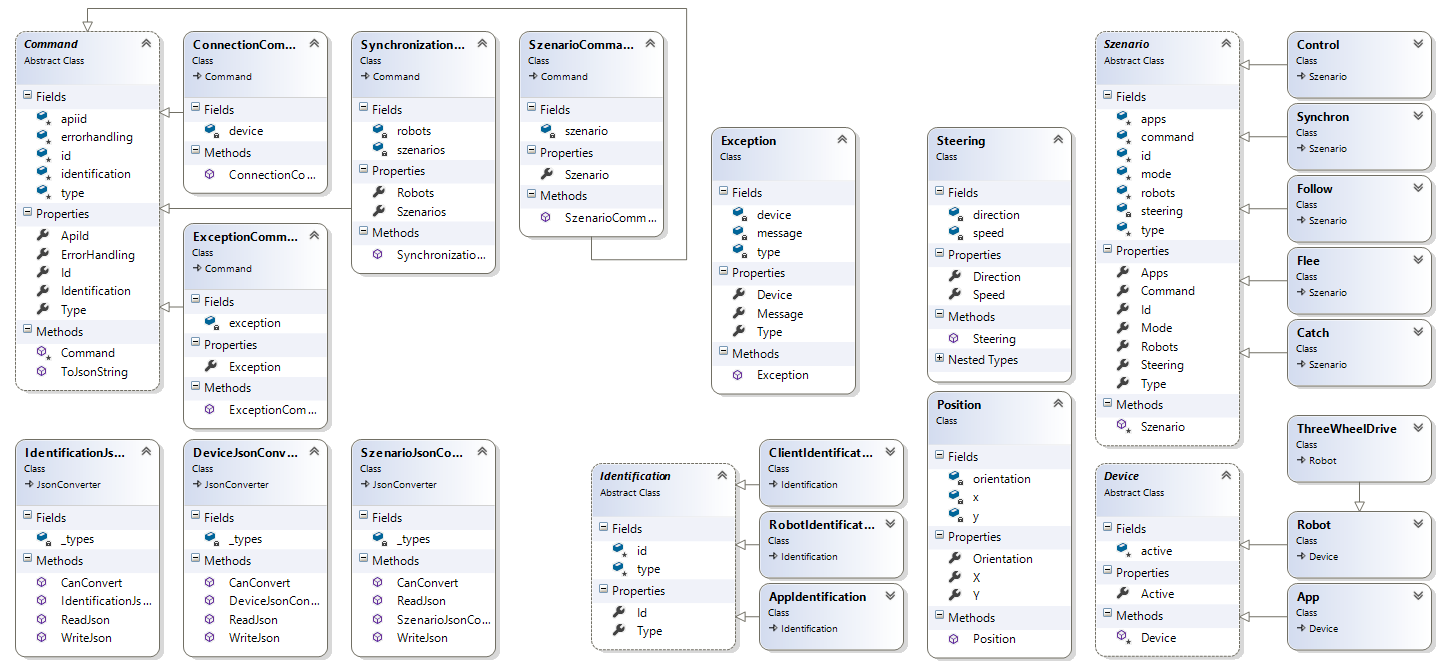
\includegraphics[width=0.95\textwidth]{images/uml/full_class_diagram.png}
	\end{center}
	\caption{Aufbau Commands}
	\label{fig:full_classdiagram}
\end{figure}

\newpage
\noindent
Der Kern zur Implementierung der Kommunikation erfolgt in zwei Methoden, die auf jeder Komponente zur Verfügung stehen. Diese dienen zum Versenden, sowie Empfangen von Daten, wobei diese als Zeichenkette serialisiert und in Bytes aufgeteilt werden, siehe Abbildung \ref{fig:SendCommand}. Um den vollständigen Umfang der Daten zu erfassen, wird die Größe ermittelt und standardmäßig mittels vier Bytes übertragen. Dadurch ist eine maximale Paketgröße von 32 Byte möglich, was einer Länge von etwa 4 Milliarden Zeichen entspricht. Die Interpretation zum Empfangen erfolgt mit ähnlichem Muster, indem zunächst die Größe der Daten festgestellt wird und die Daten deserialiert werden, siehe Abbildung \ref{fig:ReceiveCommand}.

\begin{figure}[h]
	\centering
	\subfloat[Versende Kommando]{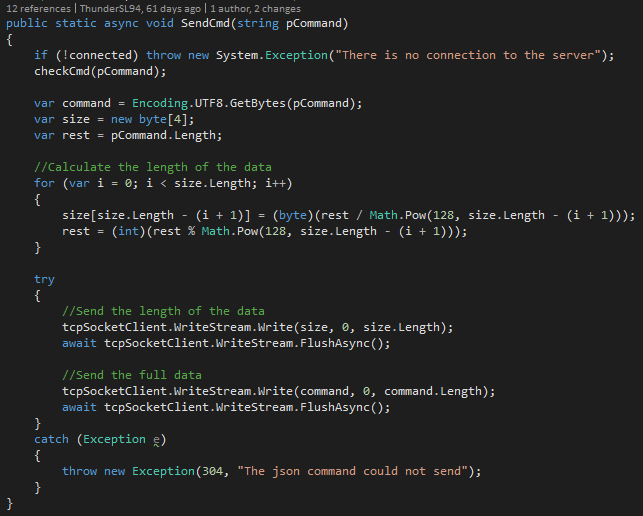
\includegraphics[width=0.6\textwidth]{images/code/SendCommand.png}\label{fig:SendCommand}}
	\qquad
	\subfloat[Empfange Kommando]{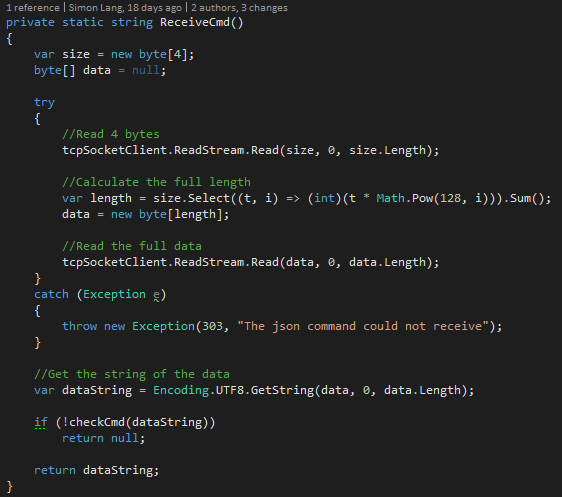
\includegraphics[width=0.6\textwidth]{images/code/ReceiveCommand.png}\label{fig:ReceiveCommand}}
	\caption{Kommunikation}
\end{figure}

\newpage
\paragraph{Kommandos}

\begin{wrapfigure}{r}{0.55\textwidth}
	\begin{center}
		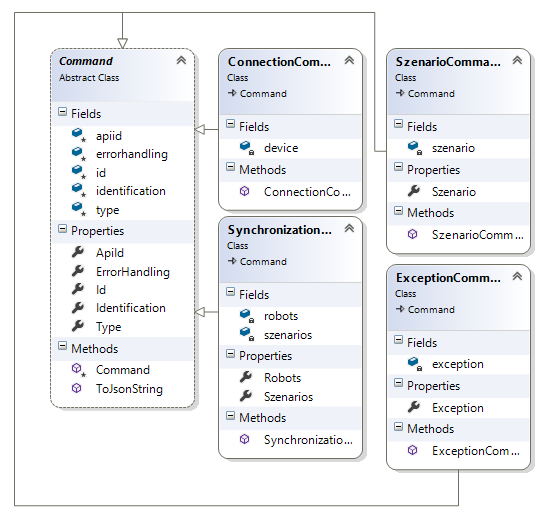
\includegraphics[width=0.5\textwidth]{images/uml/commands.png}
	\end{center}
	\caption{Kommandos}
	\label{fig:commands_classdiagram}
	\begin{center}
		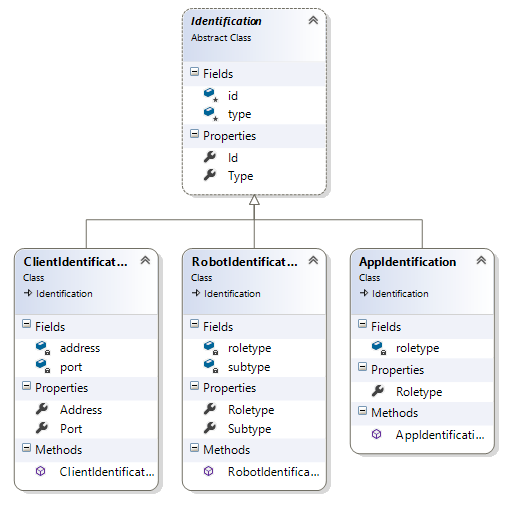
\includegraphics[width=0.5\textwidth]{images/uml/identification.png}
	\end{center}
	\caption{Identifikation}
	\label{fig:identification_classdiagram}
\end{wrapfigure}

stellen die Basis der Kommunikationsstruktur sowie den aktuellen Kontext dar, indem sich die Software befindet, siehe Abbildung \ref{fig:commands_classdiagram}. Sie enthalten grundlegende Attribute zur allgemeinen Identifikation des Kommandos, die zur Interpretation verwendet, welche über definierte Enums ausgewählt werden. Je nach Kommando sind zusätzliche Objekte enthalten, die durch die jeweilige Id vordefiniert sind.\\

\paragraph{Identifikationen}

stellt die individuelle Identität der einzelnen Komponente dar, siehe Abbildung \ref{fig:identification_classdiagram}. Diese wird durch eine fortlaufende Identifikationsnummer, Typen und je nach Ableitung weiteren Attributen erreicht. Um die jeweiligen Kommandos entsprechend zuzuordnen, sind diese in jedem Kommando vorhanden und bilden die Basisobjekte. Die unterschiedlichen Typen sind dabei für verschiedene Kontexte der Software zuständig. Die ClientIdentification stellt einerseits die Verbindung einer allgemeinen Komponente zur Desktopanwendung dar, wogegen die Robot- bzw. AppIdentification die spezifische Identifikation der Komponente darstellt. Die Erstellung der Identifikation erfolgt wiederholt zur Anmeldung der Komponente am System. Zunächst wird ein leeres Objekt erzeugt, dass anschließend durch abfragende Kommandos an die entsprechende Komponente befüllt wird, welche hinterher eine berechnete Identifikationsnummer erhält.

\newpage
\paragraph{Geräte}

\begin{wrapfigure}{r}{0.55\textwidth}
	\begin{center}
		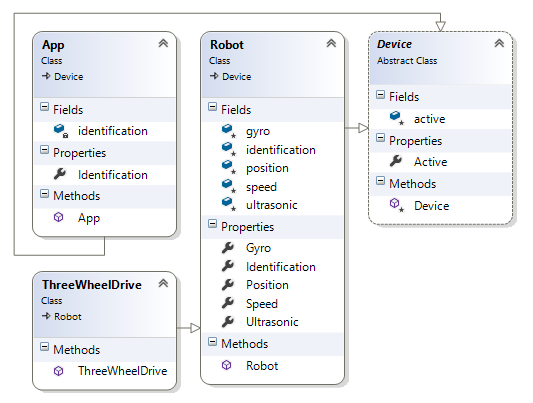
\includegraphics[width=0.5\textwidth]{images/uml/devices.png}
	\end{center}
	\caption{Devices}
	\label{fig:devices_classdiagram}
	\begin{center}
		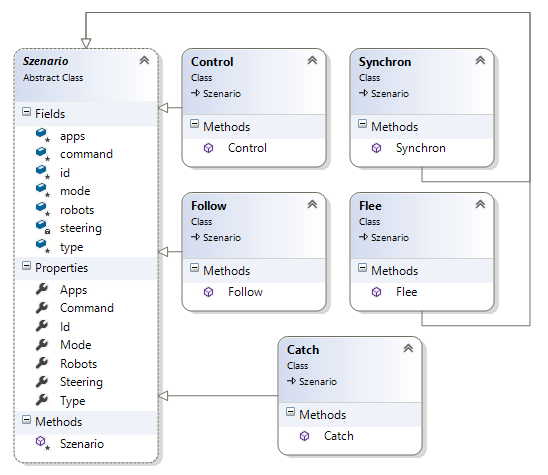
\includegraphics[width=0.5\textwidth]{images/uml/szenarios.png}
	\end{center}
	\caption{Scenarios}
	\label{fig:szenarios_classdiagram}
\end{wrapfigure}

stellen die Komponenten dar, die an einem Szenario eines Schwarmverhaltens teilnehmen, siehe Abbildung \ref{fig:devices_classdiagram}. Sie enthalten jeweils spezifische Identifikations Objekte, zur gegenseitigen Zuordnung, sowie die erfassten Daten der entsprechenden Systeme. Die Unterscheidung erfolgt in zwei Komponenten, dem Robot und der App, wobei der Roboter in die jeweiligen Untertypen gegliedert werden kann. 

\paragraph{Szenarios}

stellen den Ablauf des Schwarmverhaltens dar, in dem sich der Nutzer befindet, siehe Abbildung \ref{fig:szenarios_classdiagram}. Sie enthalten die jeweiligen Teilnehmer des Szenarios, sowie die Steuerungsinformationen und damit die gesamten Daten des aktuellen Kontextes. Diese Objekte werden laufend aktualisiert und besitzen lediglich zur Laufzeit des Szenarios ihre Gültigkeit. Dabei existieren verschiedene Kategorien von Szenarien, siehe Abschnitt \ref{szenarien}. Diese definieren jeweils einen unterschiedlichen Kontext und besitzen daher je nach Szenario zusätzliche Attribute.

\newpage
\paragraph{Konverter}

\begin{wrapfigure}{r}{0.55\textwidth}
	\begin{center}
		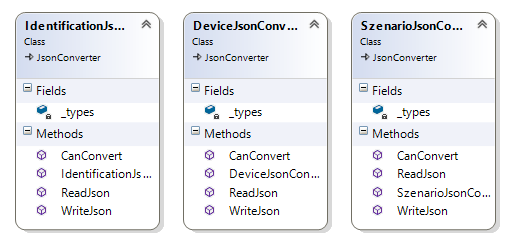
\includegraphics[width=0.5\textwidth]{images/uml/json_converter.png}
	\end{center}
	\caption{JsonConverter}
	\label{fig:converter_classdiagram}
\end{wrapfigure}

dienen der Deserialisierung von abstrakten \gls{json} Objekten, welche nicht direkt identifiziert werden können, siehe Abbildung \ref{fig:converter_classdiagram}. Dazu gehören abstrakte Klassen, sowie Schnittstellen, welche keinem spezifischen Objekt zugeordnet werden kann. Die Implementierung erfolgt durch die Überschreibung der entsprechenden Methoden zur Deserialisierung und Serialisierung, siehe Abbildung \ref{fig:ConverterRead} und \ref{fig:ConverterWrite}. Je nach Anwendung, wird ein Parameter übergeben, der das Objekt als Zeichenkette beinhaltet. Dieses wird durch eine Abfolge von Bedingungen auf den Typen geprüft wird, um das Objekt zu erstellen.\\

\begin{figure}[h]
	\centering
	\subfloat[ReadJson]{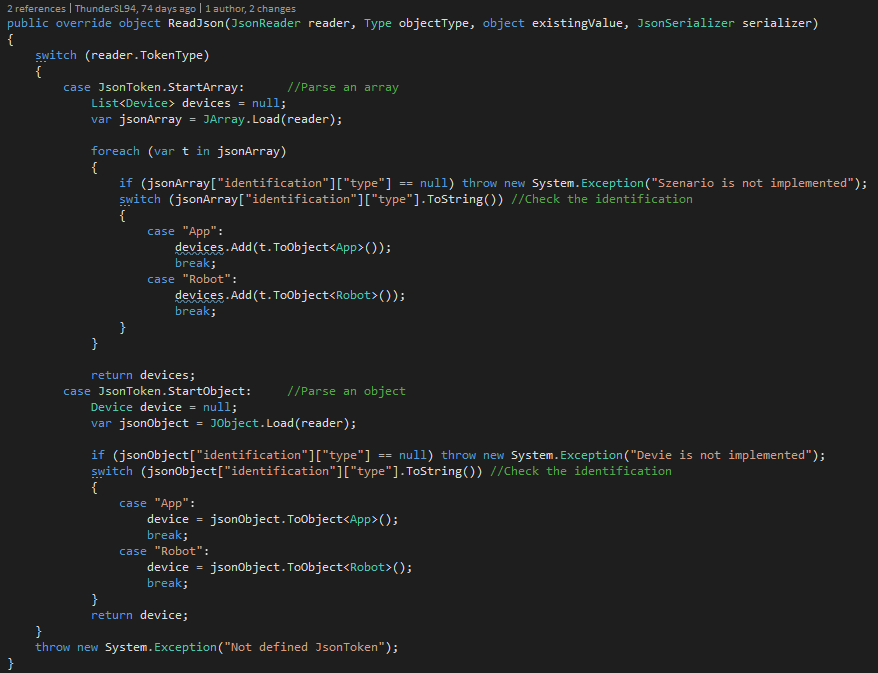
\includegraphics[width=0.6\textwidth]{images/code/DeviceConverterRead.png}\label{fig:ConverterRead}}
	\qquad
	\subfloat[WriteJson]{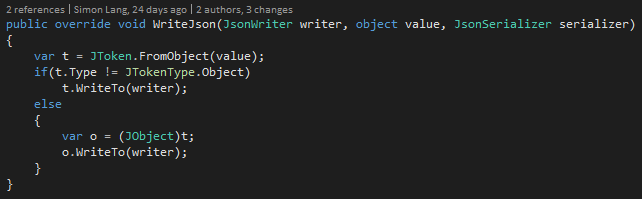
\includegraphics[width=0.6\textwidth]{images/code/DeviceConverterWrite.png}\label{fig:ConverterWrite}}
	\caption{Device JsonConverter}
\end{figure}

\newpage
\subsection{\gls{app}}

Die Erstellung der App erfolgt in einer plattformübergreifenden Implementierung durch Xamarin in C\#. Kernelemente stellen hierbei die Struktur, Oberfläche, Businesslogik sowie das Kommunikationssystem dar. Durch die zentrale Verwendung des Kommunikationssystems wird dieses in ein separates Projekt untergliedert, siehe Abbildung \ref{fig:solution} und wird als solches von der \gls{app} als Bibliothek eingebunden. Somit lässt sich die Logik einmalig implementieren und kann auf andere Systemen entsprechend übertragen werden.\\
Die \gls{app} setzt sich aus vier verschiedenen Projekten zusammen, einer \acrshort{pcl} als Projekt zur plattformübergreifenden Entwicklung und den plattformspezifischen Projekten. Diese werden dem Zielsystem entsprechend ausgewählt und erzeugen durch ihre bestehende Referenz auf die \acrshort{pcl} einen plattformspezifischen Quellcode als \gls{il}, der anschließend ausgeführt werden kann.\\

\begin{figure}[h]
	\begin{center}
		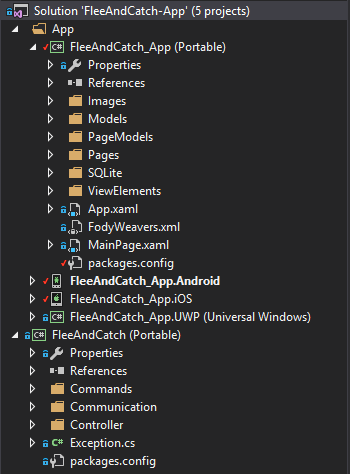
\includegraphics[width=0.5\textwidth]{images/implementation/solution.png}
	\end{center}
	\caption{Projektstruktur}
	\label{fig:solution}
\end{figure}

\newpage
\subsubsection{Workflow} %Struktur

Die Struktur der \gls{app} basiert auf dem in Xamarin verbreiteten Design Pattern \acrlong{mvvm}, welches durch ein Benachrichtigungssystem zwischen den verschiedenen Strukturen der \gls{app} eine Abspaltung der Daten, \gls{gui} und dem Businesscode erlaubt. Zusätzlich wird die standardmäßig vorhandene CodeBehind Struktur der einzelnen Seiten verwendet, wobei der Businesscode an das Layout der Seite gebunden ist, um diese miteinander zu verbinden. Zur lokalen Speicherung der Daten wird SQLite durch eine implementierte Schnittstelle verwendet, welche plattformübergreifend ansprechbar ist.

\paragraph{\acrfull{mvvm}}

stellt ein Design Pattern dar, welches eine grundlegende Struktur im Quellcode ermöglicht, siehe Abbildung \ref{fig:mvvm}. Dabei wird die erstellte Benutzeroberfläche von der Logik, sowie den Daten getrennt, um Änderungen unabhängig voneinander durchführen zu können. Die einzelnen Objekte werden dabei durch Referenzen verbunden um diese durch Events entsprechend zu aktualisieren.\\

\begin{tabular}{p{2.5cm} p{12.25cm}}
	\textbf{Model:} & Datenschicht, welche durch den Benutzer über die \gls{gui} verändert werden kann und über Datenänderungen die entsprechenden Elemente benachrichtigt \\
	\textbf{View:} & \gls{gui} mit den anzuzeigenden Elementen, welche an das ViewModel gebunden sind und der Benutzerinteraktion dienen. \\
	\textbf{ViewModel:} & Logik des \gls{ui} als zentrale Schnittstelle zwischen dem Model und der View zum Austausch von Informationen, indem entsprechende Methoden und Dienste ausgeführt werden. \\
\end{tabular}

\bigskip

\begin{figure}[h]
	\begin{center}
		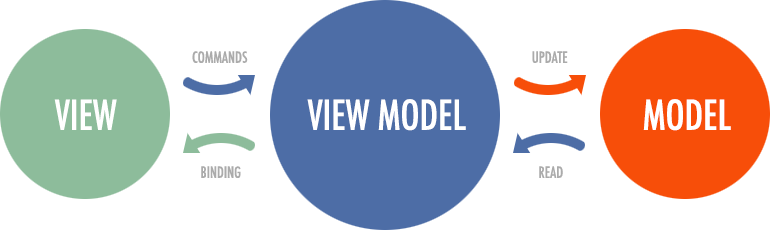
\includegraphics[width=0.95\textwidth]{images/implementation/mvvm.png}
	\end{center}	
	\caption{\acrlong{mvvm} \cite{Brecht.MVVMEntity}}
	\label{fig:mvvm}
\end{figure}

\newpage
\subsubsection{\acrfull{gui}} %Oberfläche

Die Oberfläche der \gls{app} wird mittels \gls{xaml} durch verschiedene von Xamarin zur Verfügung gestellten Elementen realisiert. Da eine \gls{app} ein einfaches Bedienkonzept voraussetzt, damit es von jedem beliebigen Benutzer verwendet werden kann,


Dabei wird für das Layout der einzelnen Seiten vor allem auf ein StackLayout gesetzt. Dieses ist sehr einfach umzusetzen, indem eine Orientierung zur Anordnung der verschiedenen Elemente festgelegt wird, welche anschließend nacheinander eingefügt werden. 




 Dabei wird für die Navigation der einzelnen Seiten vor allem auf die Verwendung der NavigationPage sowie zur Auswahl des Szenarios auf ein Carousel gesetzt. 




 mit den Aufbau eines STacks durch pushund pop aufrufe die entsprechenden Seiten gewechselt werden, siehe Abbildung xx. 

\begin{comment}
	Die Oberfläche der \gls{app} wird mittels \gls{xaml} realisiert. Dabei werden die einzelnen Elemente untereinander in der typischen \gls{xml} Struktur angeordnet und stellen damit die \gls{gui} dar, welche die einzelnen Elemente zur Benutzerinteraktion beinhaltet. Zur Strukturierung des Design bietet Xamarin verschiedene Arten von Layouts, wobei diese \gls{app} auf die Stacklayout zur Struktureirung und einer NavigationPage zur Naviagtion, sowie einem Carousel der Szenario auswahl setzt.
\end{comment}

\begin{comment}
	Die Oberfläche der \gls{app} wird mittels XAML erstellt, welche auf der Basis von XML ist. Dabei werden die einzelnen ELemente untereinnander Strukturuert, wobei der ENtwickler in Xamarin verschiedene Möglichkeiten des Designs besitzt. Grundlegend ist die entscheidung, ob eine plattformspezifisches Design sinnn macht, oder aber ein plattformübergreifendes, wobei dieses weniger Freiheiten bietet. Die plattformübergreifendes Design besitzt eine Reihe von grundlegeneden Layouts, die für Xamamrin eingesetzt werden können, sowie unterschiedliche Seitenarten. Views
	Seiten (ContentPage, MasterDetailPage, NavigationPage, TabbedPage, TemplatedPage, CaruselPage)
	View (ContentPresenter, ContentVIew, ScrollVIew, Frame, TemplatedVIew)
	Layout (Stacklayout, absolutLayout, RelativeLayout, GridLayout)
	
	Weitere standardelemente
	
	Durch verschiednene Packages könenn dabei viele Zusätzliche DInge erstellt werden
\end{comment}


%General, XAML stuff

\begin{figure}[h]
	\begin{center}
		
\includegraphics[width=0.75\textwidth]{images/implementation/push.png}
	\end{center}	
	\caption{Wechsel auf neue Seite}
	\label{fig:push}
	\begin{center}
		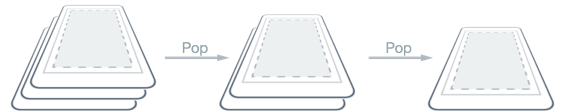
\includegraphics[width=0.75\textwidth]{images/implementation/pop.png}
	\end{center}	
	\caption{Wechsel auf alte Seite}
	\label{fig:pop}
\end{figure}

\paragraph{SignIn Page} stellt die Benutzerschnittstelle zur Anmeldung des Nutzers am System dar, siehe Abbildung \ref{fig:signin}. Dabei gibt dieser die entsprechende IP-Adresse der laufenden Desktopanwendung zur Verbindung an. Durch eine implementierte Logik wird diese IP-Adresse auf ihre Richtigkeit geprüft und die Verbindung gestartet. Bei einer erfolgreichen Verbindung wird der Benutzer zur \gls{app} weitergeleitet, wodurch ihm die entsprechenden Funktionalitäten zur Verfügung stehen. Andernfalls erscheint nach einem definierten Timeout eine Fehlermeldung, welche dem User Informationen vorlegt. Zur Speicherung der IP-Adresse ist zusätzlich die Möglichkeit durch ein Switch Element gegeben, wobei diese bei Start der \gls{app} automatisch eingefügt wird.

\begin{figure}[h]
	\begin{center}
		
\includegraphics[width=0.4\textwidth]{images/implementation/signin.png}
	\end{center}	
	\caption{SignIn Page}
	\label{fig:signin}
\end{figure}

\paragraph{Home Page} stellt die Hauptseite mit der grundlegenden Navigation der \gls{app} dar, indem der Benutzer die Möglichkeit besitzt ein neues Szenario eines Schwarmverhaltens zu starten, Informationen über die \gls{app} abzurufen, oder sich vom aktuelles System abzumelden.

\begin{figure}[h]
	\begin{center}
		
\includegraphics[width=0.4\textwidth]{images/implementation/home.png}
	\end{center}	
	\caption{Home Page}
	\label{fig:home}
\end{figure}

\newpage
\paragraph{Option Page} stellt die Benutzerschnittstelle dar, welche diesen durch die vorhandenen Szenarien anhand eines Carousels leitet und ein entsprechends auswählt.

\begin{figure}[h]
	\begin{center}
		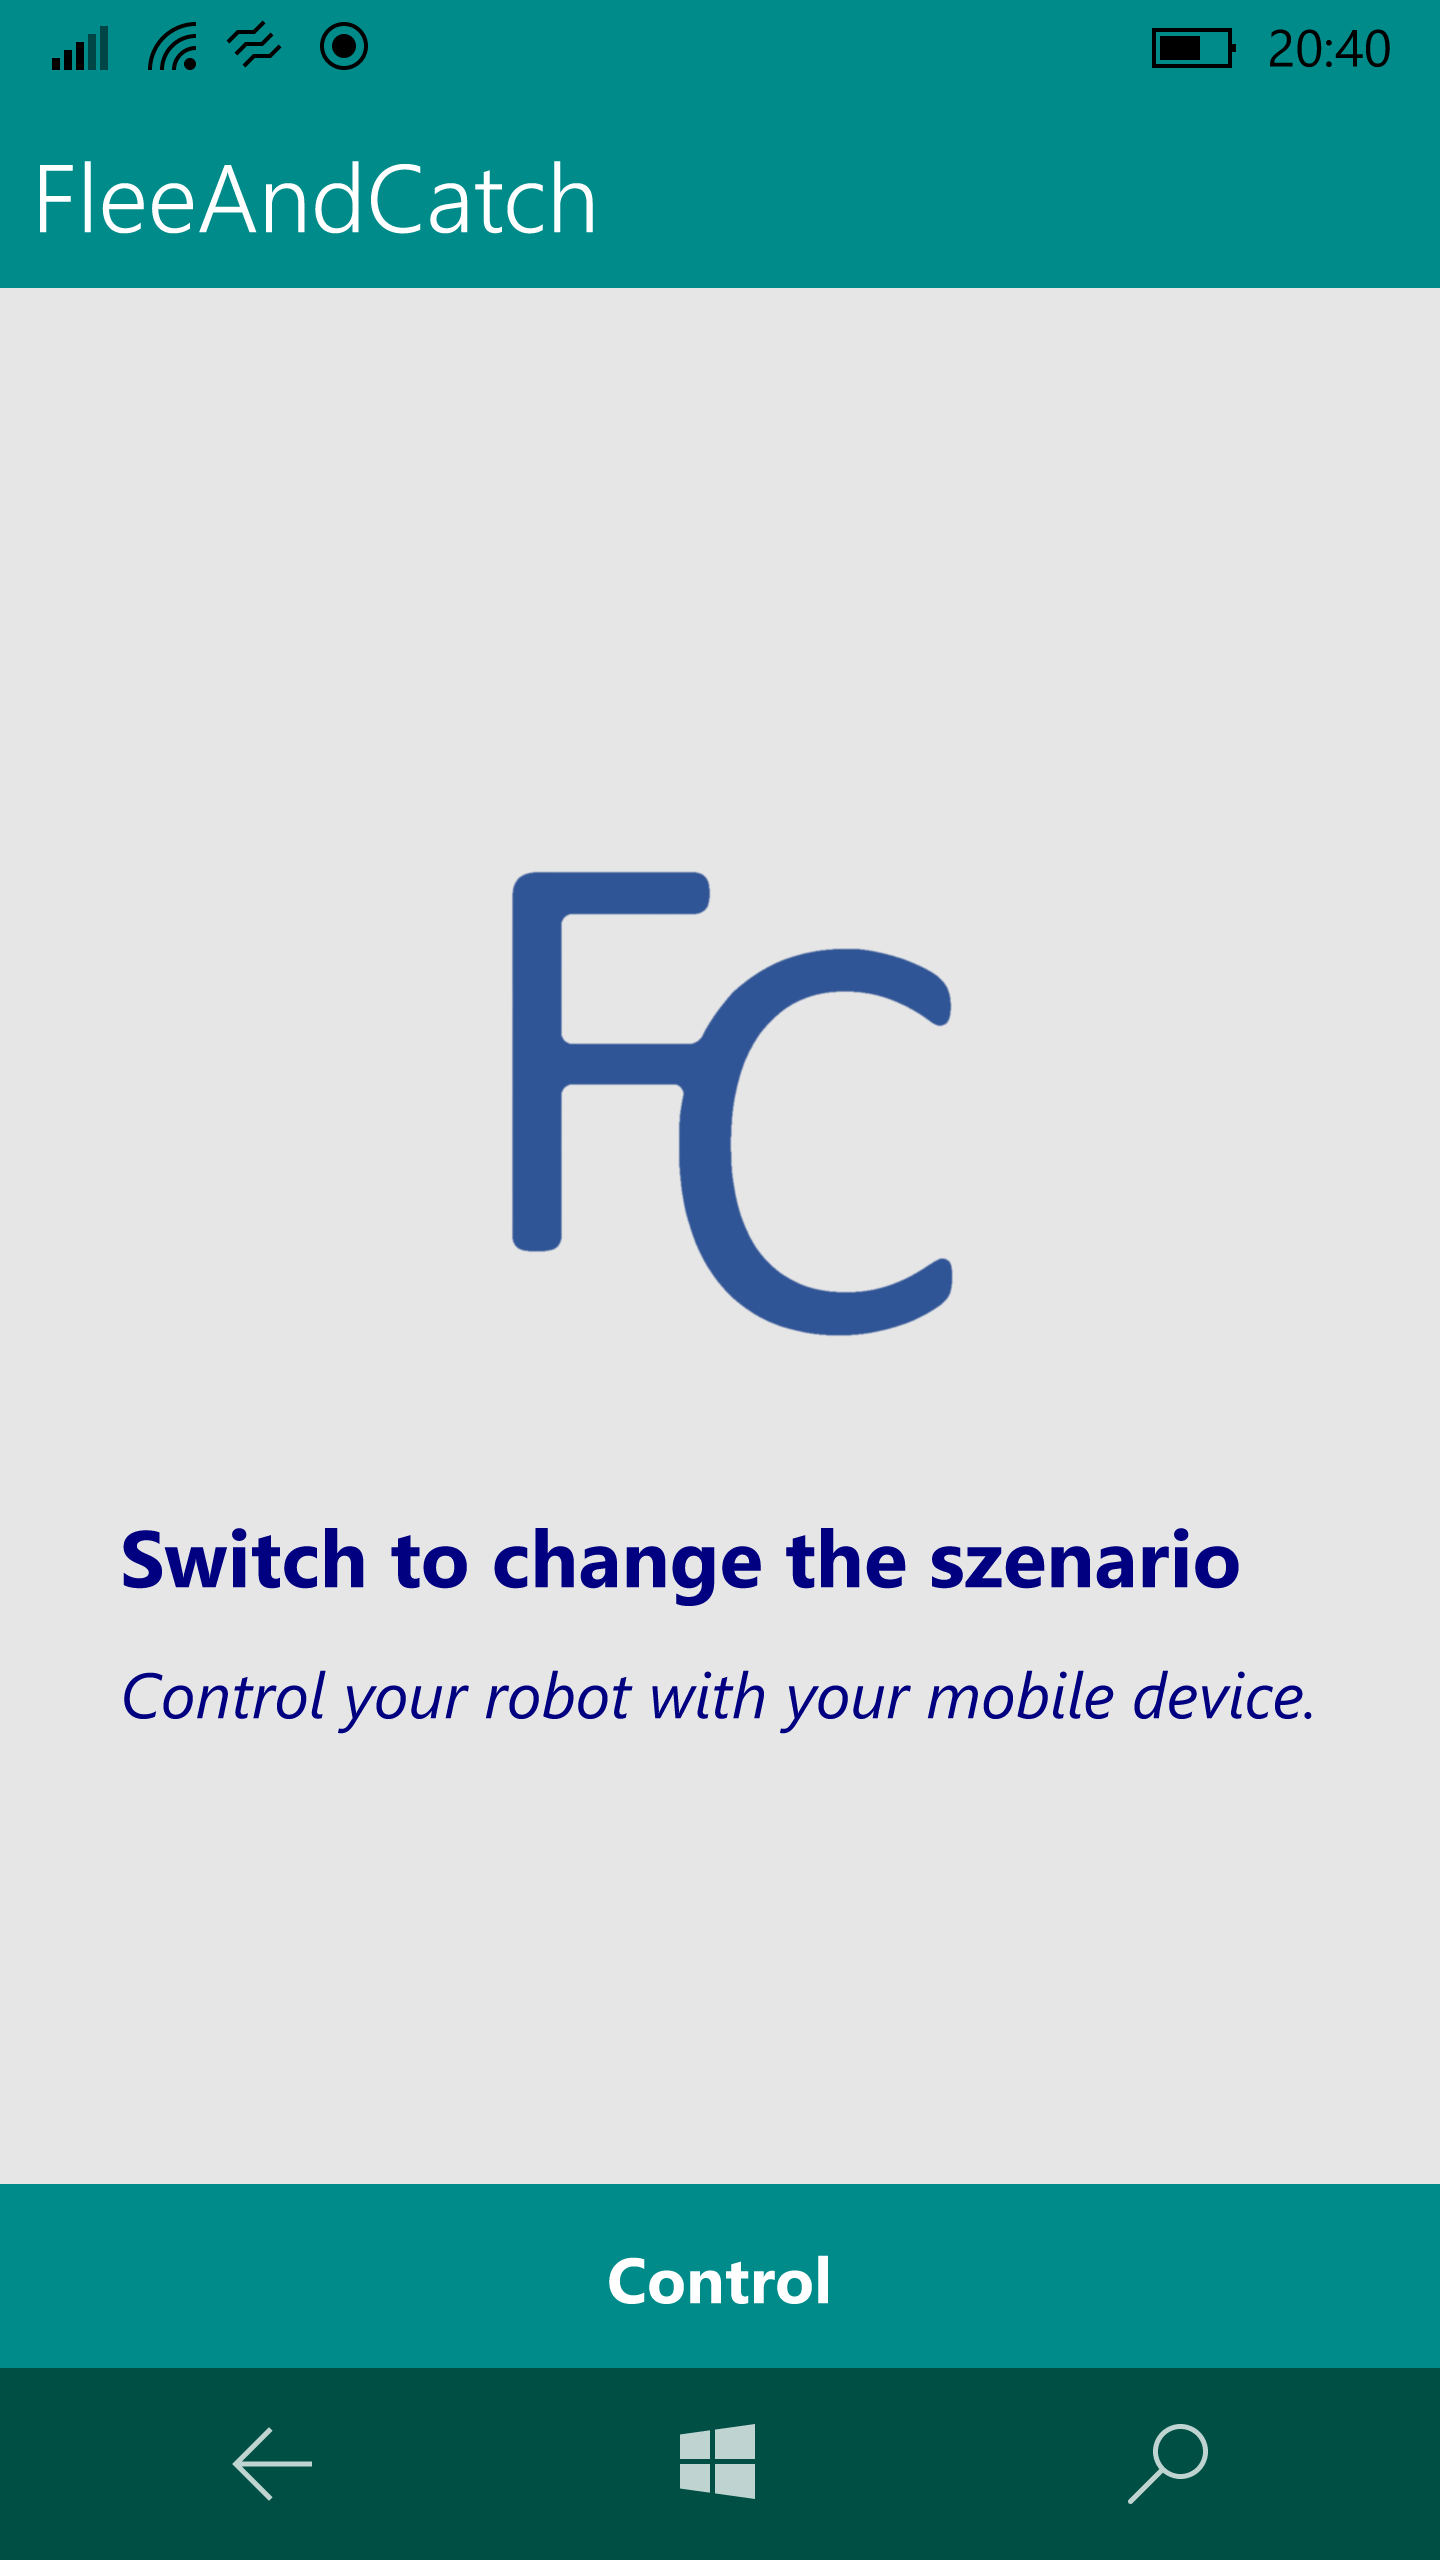
\includegraphics[width=0.4\textwidth]{images/implementation/option.png}
	\end{center}	
	\caption{Option Page}
	\label{fig:option}
\end{figure}

\newpage
\paragraph{List Page} stellt die Benutzerschnittstelle zur Auswahl der Robotern, welche im Szenario involviert werden sollen. Dabei kann der Benutzer unter den verschiedenen Typen wählen, welche vorhanden sind, wobei die Anzahl der Roboter vom gewählten Szenario abhängt.

\begin{figure}[h]
	\begin{center}
		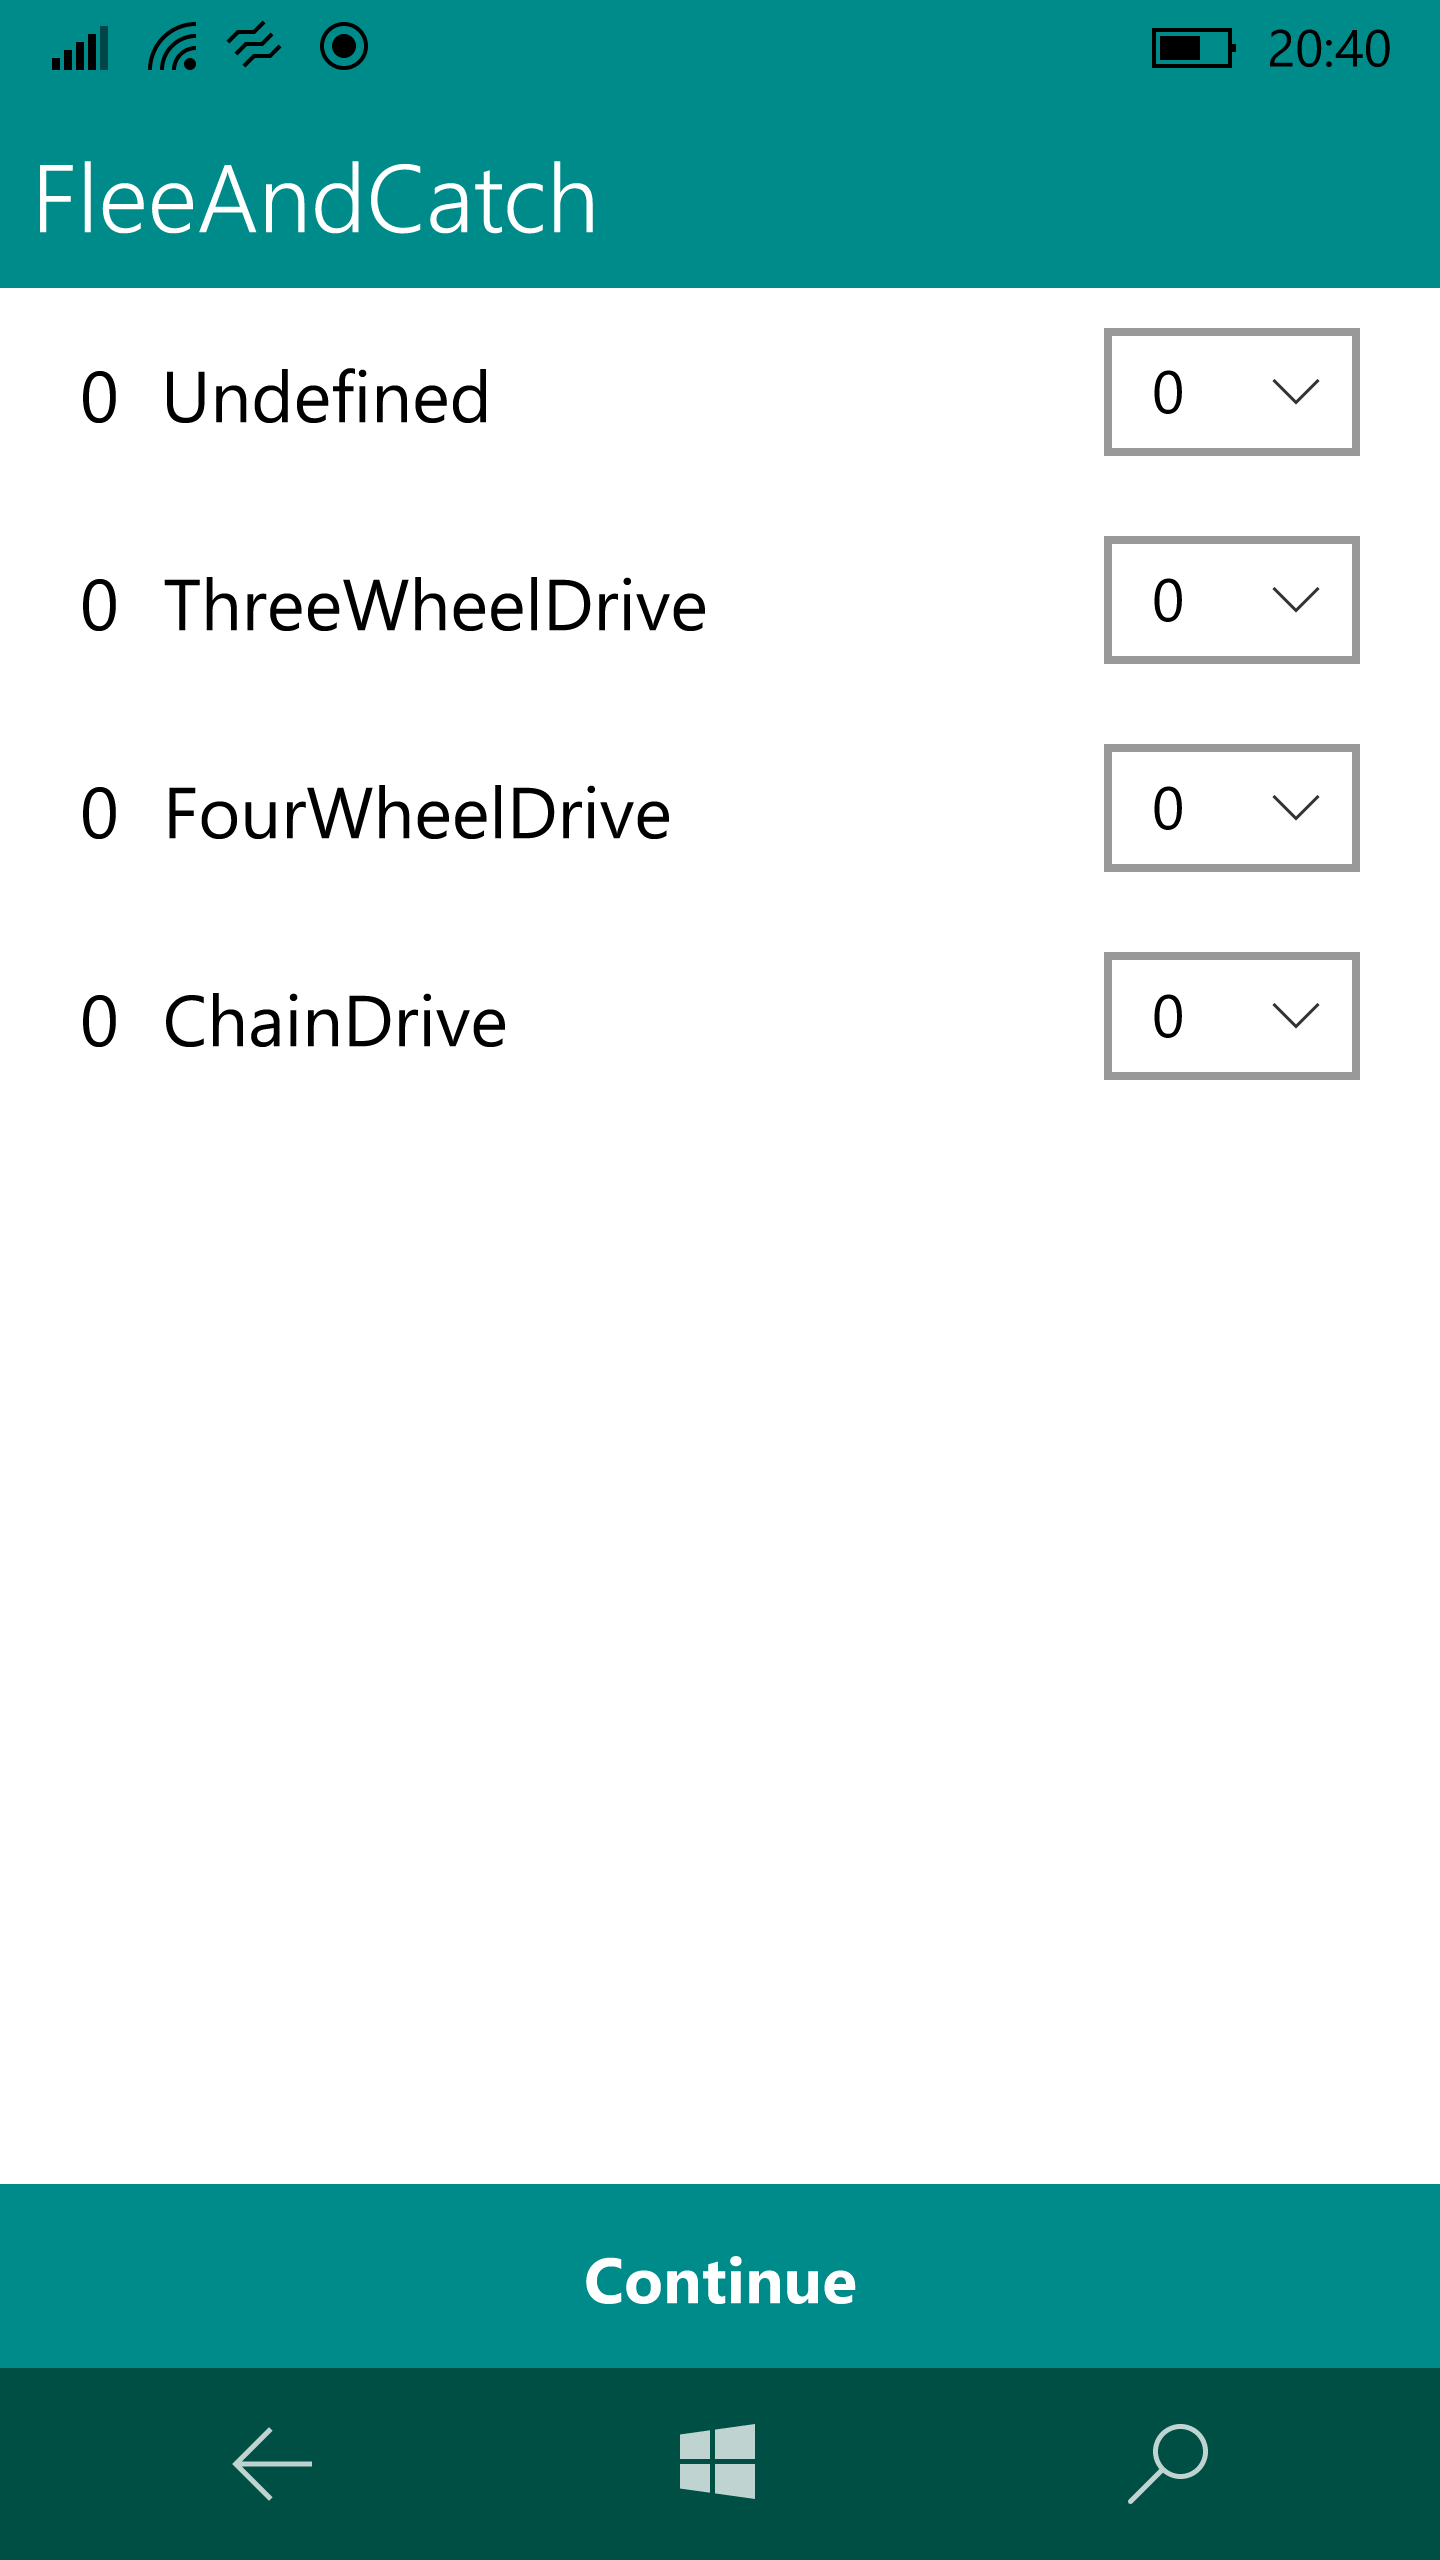
\includegraphics[width=0.4\textwidth]{images/implementation/list.png}
	\end{center}	
	\caption{List Page}
	\label{fig:list}
\end{figure}

\newpage
\paragraph{Szenario Page} stellt die Benutzerschnittselle dar, die einerseits der Steuerung und Überwachung des Schwarmverhaltens dient. Dabei werden laufend die aktuellen Daten der Roboter angezeigt und können durch die Neigungssensoren der eräte gesteuert werden. Diese verhalten sich entsprechend dem ausgewählten SZenario.

\begin{figure}[h]
	\begin{center}
		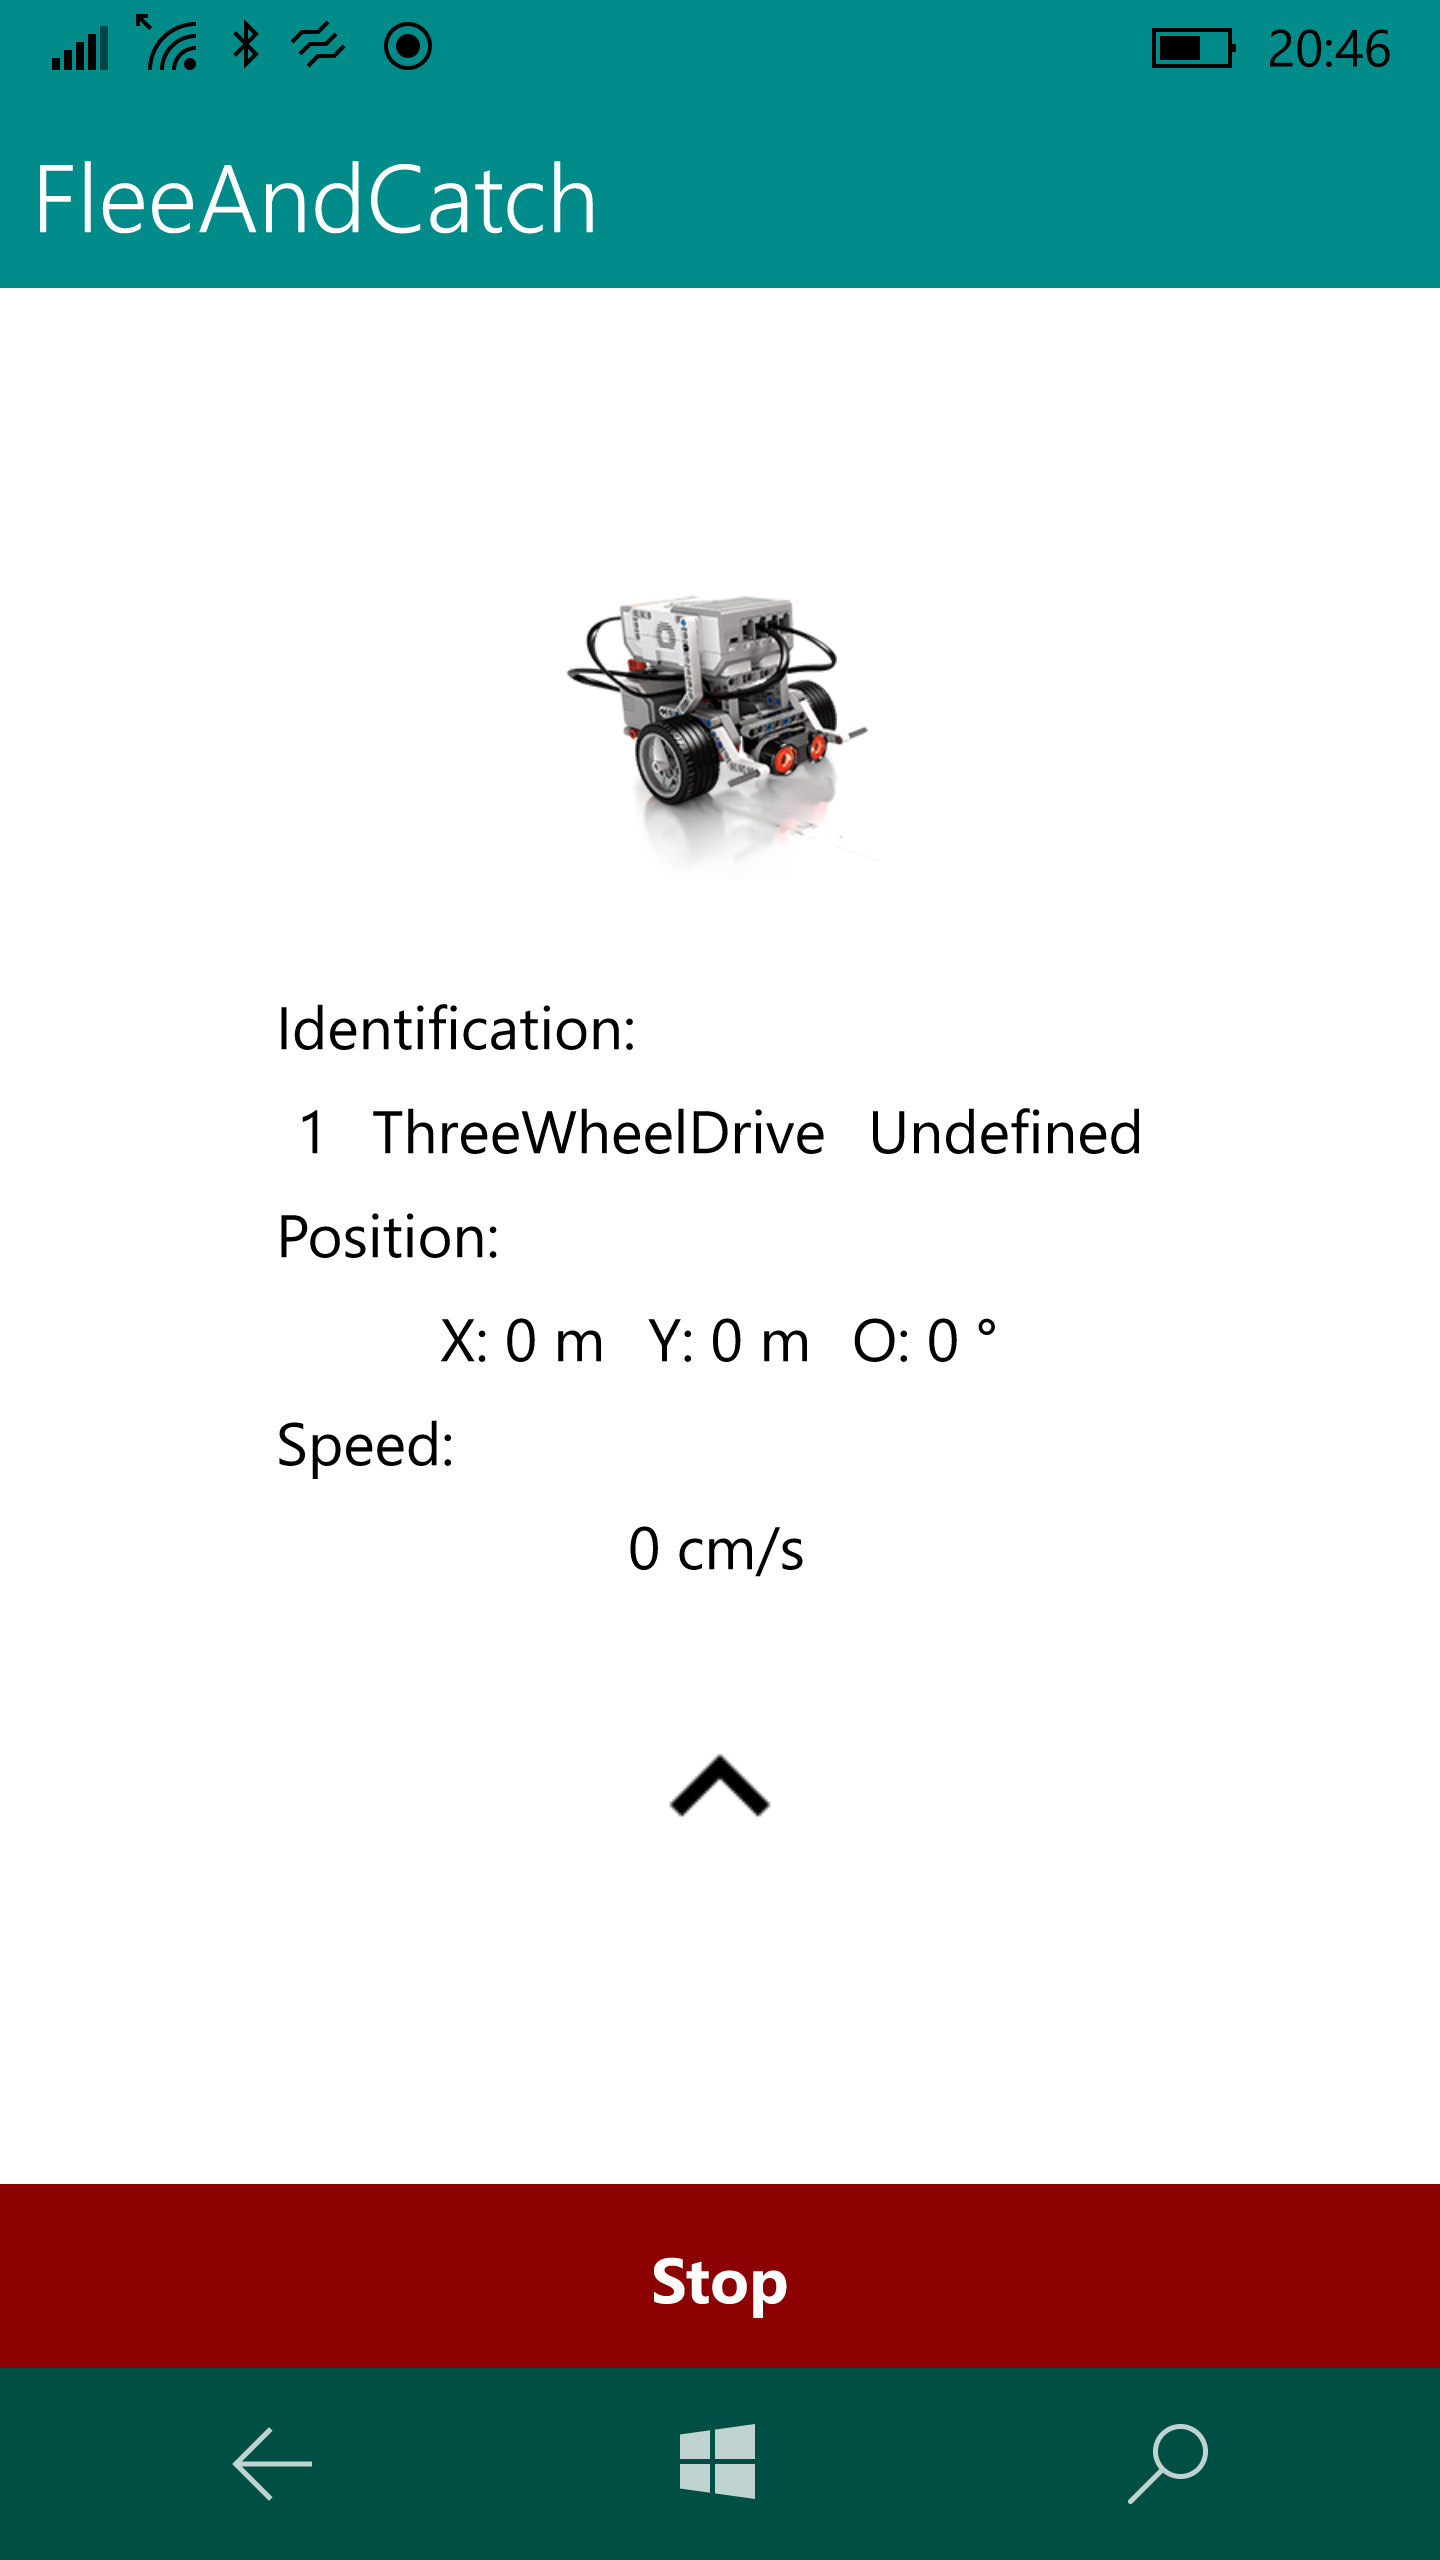
\includegraphics[width=0.4\textwidth]{images/implementation/szenario.png}
	\end{center}	
	\caption{Szenario Page}
	\label{fig:szenario}
\end{figure}

\newpage
\subsubsection{Buisnesslogic} %Logik

\paragraph{Authorization}

\paragraph{Create Szenario}

\paragraph{Szenario}

\newpage
\subsection{Backend}
Das Backend ist die Kommunikations- und Verwaltungszentrale des Projekts und bildet das Rückgrat der Kommunikation. Es verwaltet die 
Devices im Kontext der einzelnen Szenarien und sorgt für den Datenaustausch zwischen den verschieden Geräten. \\
Realisiert ist des Backend wie auch der Roboter in der Programmiersprache Java. Das bringt neben der plattformunabhängigen 
Lauffähigkeit des Programms noch weitere Vorteile mit sich. So können vor allem Programmkomponenten welche die Kommunikation und
den Datenaustausch betreffen für die Roboter- bzw. Backend-Implementierung wiederverwendet werden und müssen nicht komplett neu
implementiert werden.
\subsubsection{Die GUI}
Neben den rein Funktionalen Komponenten des Backends verfügt dieses auch über eine grafische Benutzeroberfläche die Informationen zu
den angemeldeten Geräten und den existierenden Szenarien zur Verfügung stellt. Diese Benutzeroberfläche ist so realisiert das diese 
komplett losgelöst von den der eigentlichen Funktionalität des Backend ist. Sie setzt lediglich auf dem eigentlichen Programm auf und
ist zu dessen Ausführung nicht notwendig. Dadurch ist es möglich das Programm komplett ohne grafische Benutzeroberfläche zu starten so
das es im Hintergrund laufen kann und lediglich als Verwaltungs- und Kommunikationsservice dient. Ob die grafische Benutzeroberfläche 
aktiviert ist oder nicht wird beim Programmstart durch entsprechenden Parametern festgelegt. \\
Der Nutzen der GUI bestand für uns hauptsächlich im Monitoring und bei der Identifikation sowie dem Aufspüren von Fehlern während der 
Entwicklung. \\
Realisiert ist die grafische Benutzeroberfläche mit dem JavaFX-Framework welches Bestandteil der Java-Bibliothek ist uns somit wie 
Java ebenfalls plattformunabhängig lauffähig ist. Zu ihrer Ansteuerung dient eine spezielle Klasse namens
>>ViewController<< welche lediglich Informationen des eigentliche Programms entgegen nimmt und an die eigentliche Benutzeroberfläche 
(View) weiterreicht sofern diese aktiviert wurde. Umgekehrt werden jedoch keine Benutzereingaben von der GUI an das Programm 
weitergereicht, sondern dienen lediglich zur Manipulation der Anzeige so das dieses komplett unabhängig ist. Lediglich das Beenden 
das kompletten Programms ist über die grafische Benutzeroberfläche möglich.
Abbildung X.X zeigt einen Screenshot der grafischen Benutzeroberfläche des Backends. \\
\\
Da die grafische Benutzeroberfläche jedoch nicht zur eigentlichen Funktionalität des Backends beiträgt soll an dieser Stelle nicht 
weiter eingegangen werden.
\begin{comment}
Aufbau
Interpreter
Mechanismen
GUI
\end{comment}

\subsection{Robot}
Die Implementierung des Roboters stellt das Kernstück bei der Realisierung dieses Projekts dar. 
\\
\\
Da eine komplett detaillierte Beschreibung des ganzen Quellcodes den Umfang dieser Ausarbeitung bei weitem sprengen würde,
werden in diesem Kapitel die wichtigsten Implementierungskonzepte deren Funktionswiese, sowie deren Komponenten dargestellt. 
Für eine vollständig detaillierte Darstellung wird auf den Quellcode und den darin enthalten Kommentare sowie das zugehörige 
github-Wiki (https://github.com/FleeAndCatch-Dev/FleeAndCatch-Docs/wiki) verwiesen.
\subsubsection{Threads}
Für die Umsetzung der Szenarien ist es erforderlich das der Roboter verschiedene Dinge parallel erledigt. Zum einen muss die 
ständige und zeitnahen Kommunikation mit dem Backend aufrecht erhalten werden, um zum einen Steuerdaten sowie die Positionsdaten
der anderen Roboter für die Bewegungsberechnung zu empfangen. Andererseits müssen über diese Verbindung die eigenen Daten übermittelt
an das Backend übermittelt werden. Darüber hinaus muss die eigentliche Steuerung des Roboters erfolgen. \\
Zur Realisierung all dieser Aufgaben sind innerhalb des Roboters die folgenden X Threads implementiert:
\begin{itemize}
	%   ###############################################################################################################################
	\item{Hauptthread (main thread)}
	%   ###############################################################################################################################
	\item{Kommunikationsthread (connectionThread)}
	%   ###############################################################################################################################
	\item{Steuerungsthread (steeringThread)}
	%   ###############################################################################################################################
	\item{Datenerfassungsthread (synchronizeThread)}
	%   ###############################################################################################################################
\end{itemize}
In den folgenden Abschnitten werden die einzelnen Threads sowie ihre Aufgaben dargestellt:
\paragraph{Hauptthread}
Der Hauptthread ist der Thread welcher beim Programmstart (Aufruf der Funktion public static void main(String[] args)) automatisch 
erzeugt wird und der immer vorhanden ist. Durch diesen Thread werden in der Initialisierungsphase alle anderen Threads die 
zur Kommunikation, Steuerung und Datenerfassung benötigt werden erzeugt. 
\paragraph{Kommunikationsthread}
\paragraph{Steuerungsthread}
Der Steuerungsthread hat wie der Name schon sagt die Aufgabe den Roboter zu steuern das heiß seine Geschwindigkeit und Bewegungsrichtung 
umzusetzen. Implementiert ist der Steuerungsthread in der RobotController Klasse die als Schnittstelle zwischen der Kommunikation und den
Roboterfunktionalitäten fungiert. \\
Die konkrete Umsetzung der Steuerung die durch diesen Thread erfolgt wird im Abschnitt X.X beschrieben.
\paragraph{Datenerfassungsthread}
Neben dem Empfangen von Daten und der Umsetzung der Steuerung muss der Roboter auch seine eigen Daten wie Position, Orientierung und 
Geschwindigkeit kontinuierlich erfassen und an das Backend übermitteln so das diese Informationen den anderen Robotern zur Verfügung
gestellt werden können. Da dieser Thread dazu auf Funktionalitäten des Roboters zugreift ist auch dieser innerhalb der RoboterController
Klasse implementiert.
\\
Die Realisierung der Datenerfassung ist weit weniger komplex als die der Steuerung des Roboters. 
Die Abbildung X.X zeigt das Zusammenspiel der einzelnen Threads bzw. den Ablauf ihrer Erzeugung und Terminierung:
\subsubsection{Klassen}
Neben den verschiedenen Threads enthält das Roboterprogramm zahlreiche Klassen durch welche die vielfältigen Funktionen abgebildet 
werden die, der Roboter zur Realisierung der verschiedenen Szenarien mitbringen muss. 
\paragraph{Klassenstruktur}
\color{finishing}             % Farbe die angibt welchen Status der folgende Abschnitt hat!
% Eigentlicher Text:
Zur Strukturierung und einer sauberen Trennung der einzelnen Klassen und ihren Sichtbarkeiten, sind diese in verschiedenen 
Paketen (Java-Packages) organisiert. Diese Klassenstruktur ist hierarchisch aufgebaut, orientiert sich an den grundlegenden 
Bestandteilen des Programms (Kommunikation, Roboterkontrolle etc.) und granuliert in einzelnen Unterpakete anhand der Objekten 
welche die jeweiligen Klassen darstellen bzw. welche Funktionen diese bieten. \\
Bei der Umsetzung wurden die Klassen in den folgenden vier großen Paketbereiche strukturiert.
\begin{itemize}
	%   ###############################################################################################################################
	\item{Kommunikation (\code{flee\_and\_catch.robot.communication})} -- Enthält sämtliche Klassen die für die Kommunikation mit dem
	Backend notwendig sind dazu zählen die Eigentlichen Kommunikator (Sockets), die verschieden Kommandos sowie serialisierbare 
	Datenobjekte.
	%   ###############################################################################################################################
	\item{Roboter (\code{flee\_and\_catch.robot.robot})} -- Hier befinden sich alle Klassen die direkten Zugriff bzw. Einfluss auf den 
	physischen Roboter haben. Dies sind hauptsächlich Sensoren, das Roboter-Interface, Klassen die einen konkreten Roboter darstellen, 
	sowie die zentrale Steuerklasse >>RoboterController<<.
	%   ###############################################################################################################################
	\item{View (\code{flee\_and\_catch.robot.view})} -- Enthält Klassen die der Anzeige d.h Ansteuerung des LCD-Displays des
	Roboters dienen. Zwar ist das LCD-Display auch Bestandteil des Roboters, es wurde sich aber für eine Trennung dieser beiden 
	Bereiche entschieden da diese möglichst unabhängig voneinander bleiben sollten.
	%   ###############################################################################################################################
	\item{Konfiguration (\code{flee\_and\_catch.robot.configuration})} -- Zentrales Paket welches Klassen zur Konfiguration 
	der verschiedenen Programmteile enthält.
	%   ###############################################################################################################################
\end{itemize}
Innerhalb dieser Hauptpakete existieren zahlreiche weitere Unterpakete welche die Klassen weiter strukturieren. Die saubere Einordnung
und Trennung der Programmklassen ermöglicht es in Verbindung mit der Festlegung entsprechender Sichtbarkeiten, die Klassen gegeneinander 
abzuschotten. So wird erreicht, dass die Programmteile lediglich über die vorgesehenen Schnittstellen miteinander interagieren und die
einzelnen Klassen nur diejenigen sehen und ansprechen können die sie tatsächlich benötigen. Zudem hilft es dem Programmierer bei der Orientierung und dem Programmverständnis.
\medskip
\newline
In den nächsten Abschnitten werden die wichtigsten Klassen und Interfaces des Programms näher beschrieben und ihre Rolle bei der 
Realisierung des durch die Roboter abgebildeten Schwarmverhaltens erläutern.
\paragraph{Das Roboter Interface}
\color{process}             % Farbe die angibt welchen Status der folgende Abschnitt hat!
% Eigentlicher Text:
Das Roboter Interface dient als Implementierungsvorlage für Klassen die einen Roboter in seiner jeweiligen physischen Gestalt d.h. mit
der jeweiligen Antriebsform, seinen verbauten Sensoren etc darstellen. Innerhalb dieses Interfaces sind sämtliche Funktionalitäten 
und Methoden definiert, die ein konkreter Roboter bzw. die entsprechende Klasse, die diesen repräsentiert implementieren muss um durch 
das Programm gesteuert und in die entsprechenden Szenarien integriert werden zu können. \\
Innerhalb dieses Interface werden dazu verschiedene Methoden zur Steuerung sowie Abfrage von Roboterparametern definiert. Die durch 
diese Methoden dargestellten Funktionalitäten sind von so grundlegender Natur das diese durch jeden Roboter realisiert bzw. umgesetzt 
werden können, wenn auch abhängig von seiner Bauart auf andere Weise. \\
Folgende Auflistung gibt einen Überblick über die wichtigsten diese Methoden und erläutert kurz die durch sie zur realisierende Funktion.
\begin{itemize}
	%   ###############################################################################################################################
	\item{\code{void forward()}} -- Soll den Roboter geradeaus vorwärts fahren lassen.
	%   ###############################################################################################################################
	\item{\code{void backward()}} -- Soll den Roboter geradeaus rückwärts fahren lassen.
	%   ###############################################################################################################################
	\item{\code{void backward()}} -- Soll den Roboter sich nach rechts oder linkes bewegen lassen abhängig von der übergebenen Richtung
	(Direction-Objekt).
	%   ###############################################################################################################################
	\item{\code{void stop()}} -- Soll den Roboter anhalten.
	%   ###############################################################################################################################
	\item{\code{void increaseSpeed()}} -- Soll die Geschwindigkeit des Roboters erhöhen (Iterativ bei jedem Aufruf).
	%   ###############################################################################################################################
	\item{\code{void increaseSpeed()}} -- Soll die Geschwindigkeit des Roboters verringern (Iterativ bei jedem Aufruf).
	%   ###############################################################################################################################
	\item{\code{boolean isMoving()}} -- Soll true zurückgeben wenn sich der Roboter bewegt.
	%   ###############################################################################################################################
	\item{\code{Position getPosition()}} -- Soll die aktuelle Position und Orientierung des Roboters in einem speziellen 
	Position-Objekt zurückgeben.
	%   ###############################################################################################################################
	\item{\code{float getRealSpeed()}} -- Soll tatsächliche (nicht eingestellte) Geschwindigkeit des Roboters zurückgeben.
	%   ###############################################################################################################################
	\item{\code{Robot getJSONRobot()}} -- Soll alle wichtigen Roboterdaten einem speziellen Roboter-Objekt zurückgeben welches 
	serialisierbar ist und damit via JSON-Objekt an des Backend übertragen werden kann.
	%   ###############################################################################################################################
\end{itemize}
Durch die Vorgaben und Verwendung dieser grundlegenden und universellen Funktionalitäten für die Programm-, Szenarien- und Steuerlogik 
ist es mögliche eine generische und flexible Implementierung zu schaffen. Da ein Roboter immer als Objekt dieses Interfaces betrachtet 
und angesprochen wird ist das restliche Programm vollkommen unabhängig von der konkreten Ausprägung des jeweilige Roboter und kennt 
diese nicht mal. Es beschränkt sich bei der Interaktion mit dem Roboter auf die in diesem Interface definierten Methoden. \\
Der Vorteil dieser Implementierung liegt darin, dass durch dieses generische Programmierung lediglich eine neuen Klasse die dieses 
Interface implementiert notwendig ist um einen neue Art von Roboter zu Realisierung und in das Projekt mit sämtlichen Szenarien zu 
integrieren. Dadurch ist das Programm leicht erweiterbar und es steigert seine Wiederverwendbarkeit. \\
Wie diese konkrete Implementierung der durch diese Methoden definierten Funktionen zu realisieren ist hängt natürlich vom jeweilige
Roboter und seinem Aufbau ab und muss durch den Programmiere entsprechend umgesetzt werden.
\paragraph{Die ThreeWheelDrive Klasse (Eine konkrete Roboter Klasse)}
\color{process}             % Farbe die angibt welchen Status der folgende Abschnitt hat!
% Eigentlicher Text:
Die Klasse >>ThreeWheelDrive<< repräsentiert den \glqq{}Standard\grqq{}-Roboter im Projekt. Sie bildet den in Abbildung X.X zu 
sehenden Roboter mit seine relevanten Komponenten wie Sensoren, Motoren sowie relevanten geometrischen und physischen Parametern ab.
Die Klasse implementiert das Roboter-Interface mit den dort definierten Methoden. 
\paragraph{Die RoboterController Klasse}
Die >>RobotController<<-Klasse übernimmt eine zentrale Rolle bei der Umsetzung der Roboter-Steuerung. Die Klasse stellt die Schnittstelle
zum physischen Roboter dar. Sämtliche Steuerkommandos und Sensorabfragen werden über diese Klasse realisiert. Durch diese einheitliche 
Schnittstelle wird es möglich die Steuerung und ... unabhängig von dem konkreten vorhandenen Roboter (Dreirädriger, Vierrädriger etc)
zu realisieren. Dazu nutzt der RoboterController intern eine Instanz des "Roboter" Interfaces was eine Ansteuerung des Roboters 
\\
Die folgende Abbildung zeigt die der verschiedenen Komponenten:
\subsubsection{Steuerung}
Eine der Hauptaufgaben des Roboterprogramms ist die Steuerung des Roboters. Dabei muss das Programm die folgende zwei 
grundlegenden Steuerungsarten unterscheiden und realisieren.
\begin{itemize}
	%   ###############################################################################################################################
	\item{Direkte Steuerung} -- Bei der direkten Steuerung erhält das Programm über das Backend von der App direkte Steuerbefehle wie
	Rechts, Links, Schneller, Langsamer welche das Programm dann in die entsprechende Bewegung des Roboters umsetzen muss.
	%   ###############################################################################################################################
	\item{Indirekte Steuerung} -- Bei der indirekten Steuerung bekommt das Programm keinen konkreten Steuerbefehle sondern muss basierend
	auf den Positionsdaten der anderen Roboter und dem vorherrschenden Szenario die notwendigen Steuerbefehle des Roboters berechnen.
	%   ###############################################################################################################################
\end{itemize}
Dabei erfolgt das Empfangen und Verarbeiten der jeweiligen Daten jeweils zyklisch in einem konfigurierbaren Zeitintervall. Beide Steuerungsarten
basieren auf dem grundlegenden Prinzip das die Daten (Steuerbefehle oder Positionsdaten) durch den X-Thread erfasst und gespeichert werden.
Der Stuerungsthread widerun liest diese Daten aus und führt die entsprechenden Roboterbefehle aus.
\paragraph{Allgemein}
\paragraph{Realisierung beim ThreeWheelDrive}
\subsubsection{Datenerfassung}
\begin{comment}
Aufbau
Robot
RobotController
EV3 Library
GUI
\end{comment}